\documentclass [a4paper, 12pt] {article}

\usepackage{syntax}
\usepackage[brazilian]{babel}
\usepackage[utf8]{inputenc}
\usepackage[light,condensed,math]{iwona}
\usepackage[T1]{fontenc}
% \usepackage[usenames, dvipsnames]{xcolor}
\usepackage[usenames, dvipsnames]{color}
% \usepackage{tgtermes} times homan font similar
\usepackage{hyperref}
\usepackage{indentfirst}
\usepackage{bbding}
% \usepackage{pifont}
\usepackage{makeidx}
\makeindex
\hypersetup{
    colorlinks,
    citecolor=black,
    filecolor=black,
    linkcolor=black,
    urlcolor=black
}
\usepackage{fullpage}
\usepackage{amssymb}
\usepackage{float}
\usepackage[toc,page]{appendix}
\usepackage{cite}
% \usepackage{draftwatermark}
% \SetWatermarkText{RASCUNHO}
% \SetWatermarkScale{1.0}
% \SetWatermarkColor[rgb]{0.9, 0.9, 0.9}

% \setdefaultlanguage[babelshorthands]{brazilian}
% \usepackage{fontspec}
% Pra mostra codigo fonte
\usepackage{listings}
\usepackage{caption}
\usepackage[most]{tcolorbox}
\DeclareCaptionFont{white}{\color{white}}
\DeclareCaptionFormat{listing}{%
  \parbox{\textwidth}{\colorbox{gray}{\parbox{\textwidth}{#1#2#3}}\vskip-4pt}}
\captionsetup[lstlisting]{format=listing,labelfont=white,textfont=white}
\lstset{frame=lrb,xleftmargin=\fboxsep,xrightmargin=-\fboxsep}

%%%  Definiciao da sintaxe da linguagem jSmall para o hiligth
\lstdefinelanguage{jSmall}{
    keywords={numfi, numf, true, false, loop, return, if, in, while, then, else, elif},
    keywordstyle=\color{blue}\bfseries,
    ndkeywords={boot, export, boolean, throw, implements, import, this},
    ndkeywordstyle=\color{darkgray}\bfseries,
    identifierstyle=\color{black},
    sensitive=false,
    comment=[l]{~},
    morecomment=[s]{~\{}{\}~},
    commentstyle=\color{purple}\ttfamily,
    stringstyle=\color{red}\ttfamily,
    morestring=[b]',
    morestring=[b]"
}

\lstset{language=C++,
    basicstyle=\ttfamily,
    keywordstyle=\color{blue}\ttfamily,
    stringstyle=\color{red}\ttfamily,
    commentstyle=\color{green}\ttfamily,
    morecomment=[l][\color{magenta}]{\#}
}

\newtcblisting[auto counter]{sexylisting}[2][]{sharp corners, 
    fonttitle=\bfseries, colframe=gray, listing only, 
    listing options={basicstyle=\ttfamily,language=jSmall, numbers=left}, 
    title=Listing \thetcbcounter: #2, #1}

\newtcblisting[auto counter]{sexylistingjava}[2][]{sharp corners, 
    fonttitle=\bfseries, colframe=gray, listing only, 
    listing options={basicstyle=\ttfamily,language=java, numbers=left}, 
    title=Listing \thetcbcounter: #2, #1}
    
\newtcblisting[auto counter]{sexylistingcpp}[2][]{sharp corners, 
    fonttitle=\bfseries, colframe=gray, listing only, 
    listing options={basicstyle=\ttfamily,language=C++, numbers=left}, 
    title=Listing \thetcbcounter: #2, #1}

% Automata packages
\usepackage{tikz, graphicx}

\usepackage{pgfplots}
\pgfplotsset{compat=1.16}
\usetikzlibrary{tikzmark, shapes.callouts}
\usetikzlibrary{automata, positioning, arrows}
\usetikzlibrary{arrows.meta, % if the figure contains arrow-tips
                bending,     % arrow tips on arcs are "bent," i.e., deformed a bit
                patterns     % if the figure contains pattern fills
               }

\usepackage{tipa}

% Hacking pra poder usar syntax package junto com o tikz
\usepackage{etoolbox}
\AtBeginEnvironment{tikzpicture}{\catcode`\_=8}

\usepackage{ifthen,xcolor,xkeyval,calc}
\newlength{\tabcont}

\newcommand{\tab}[1]{%
\settowidth{\tabcont}{#1}%
\ifthenelse{\lengthtest{\tabcont < .25\linewidth}}%
{\makebox[.25\linewidth][l]{#1}\ignorespaces}%
{\makebox[.5\linewidth][l]{#1}\ignorespaces}%
}%

\frenchspacing

% \title{
%     \textbf{\Large UNIVERSIDADE FEDERAL DE ALAGOAS}\\
%     \textbf{\Large INSTITUTO DE COMPUTAÇÃO}\\
%     {\ }\\
%     \textbf{\Large Slam Combinando}\\
%     \textbf{\Large com Filtros de Kalman}\\
%     \textbf{\Large para Robôs Móveis}\\
%     % \line(1,0){250} \\
% }
\author{Joilnen Leite\\ 2017.2}

% \usepackage[colorinlistoftodos]{todonotes}\setlength{\marginparwidth}{3cm}\reversemarginpar
\usepackage {todonotes}\setlength{\marginparwidth}{3cm}\reversemarginpar

% HACK: set length so that the paper can have better width for margin

\usepackage{float}

\usepackage{tikzscale}
\usetikzlibrary{trees,shapes.misc}
\usepackage{hologo}
\usepackage{fancyvrb}
\usepackage{listingsutf8}
\usepackage{xcolor}
\usepackage{booktabs}
\usepackage[most]{tcolorbox}
\usepackage[edges]{forest}
\definecolor{folderbg}{RGB}{124,166,198}
\definecolor{folderborder}{RGB}{110,144,169}
\newlength\Size
\setlength\Size{4pt}
\tikzset{%
  folder/.pic={%
    \filldraw [draw=folderborder, top color=folderbg!50, bottom color=folderbg] (-1.05*\Size,0.2\Size+5pt) rectangle ++(.75*\Size,-0.2\Size-5pt);
    \filldraw [draw=folderborder, top color=folderbg!50, bottom color=folderbg] (-1.15*\Size,-\Size) rectangle (1.15*\Size,\Size);
  },
  file/.pic={%
    \filldraw [draw=folderborder, top color=folderbg!5, bottom color=folderbg!10] (-\Size,.4*\Size+5pt) coordinate (a) |- (\Size,-1.2*\Size) coordinate (b) -- ++(0,1.6*\Size) coordinate (c) -- ++(-5pt,5pt) coordinate (d) -- cycle (d) |- (c) ;
  },
}
\forestset{%
  declare autowrapped toks={pic me}{},
  declare boolean register={pic root},
  pic root=0,
  pic dir tree/.style={%
    for tree={%
      folder,
      font=\normalsize,
      grow'=0,
    },
    before typesetting nodes={%
      for tree={%
        edge label+/.option={pic me},
      },
      if pic root={
        tikz+={
          \pic at ([xshift=\Size].west) {folder};
        },
        align={l}
      }{},
    },
  },
  pic me set/.code n args=2{%
    \forestset{%
      #1/.style={%
        inner xsep=2\Size,
        pic me={pic {#2}},
      }
    }
  },
  pic me set={directory}{folder},
  pic me set={file}{file},
}

\def\Size{4pt}
\tikzset{
  folder/.pic={
    \filldraw[draw=folderborder,top color=folderbg!50,bottom color=folderbg]
      (-1.05*\Size,0.2\Size+5pt) rectangle ++(.75*\Size,-0.2\Size-5pt);  
    \filldraw[draw=folderborder,top color=folderbg!50,bottom color=folderbg]
      (-1.15*\Size,-\Size) rectangle (1.15*\Size,\Size);
  },
  file/.pic={%
    \filldraw [draw=folderborder, top color=folderbg!5, bottom color=folderbg!10] (-\Size,.4*\Size+5pt) coordinate (a) |- (\Size,-1.2*\Size) coordinate (b) -- ++(0,1.6*\Size) coordinate (c) -- ++(-5pt,5pt) coordinate (d) -- cycle (d) |- (c) ;
  },
}

\newtcolorbox[blend into=tables]{mytable}[2][]{%
    enhanced,
    float, 
    every float=\centering,
    capture=hbox, 
    title = #2, 
    attach boxed title to top left={%
        xshift=5mm, 
        yshift=-\tcboxedtitleheight/2, 
        yshifttext=-1mm},
    boxed title style={colback=blue!30, sharp corners},
    colframe = gray,
    colback = blue!20, boxrule = 0.5pt,
    % overlay = {\node[text=white, fill=red] at (frame.east) 
    %     {$\clubsuit$};},
    #1}

% \definecolor{codegreen}{rgb}{0,0.6,0}
\definecolor{codebrown}{rgb}{.6,.3,0}
\definecolor{codegray}{rgb}{0.5,0.5,0.5}
\definecolor{codepurple}{rgb}{0.58,0,0.82}
\definecolor{backcolour}{rgb}{0.95,0.95,0.92}

\DeclareEmphSequence{\bfseries, \mdseries}
% \renewcommand{\baselinestretch}{0.5}

\lstdefinestyle{mystyle}{
    backgroundcolor=\color{backcolour},   
    % commentstyle=\color{codebrown},
    commentstyle=\color{black},
    keywordstyle=\color{magenta},
    numberstyle=\tiny\color{codegray},
    stringstyle=\color{codepurple},
    basicstyle=\ttfamily\tiny,
    breakatwhitespace=false,         
    breaklines=true,                 
    captionpos=b,                    
    keepspaces=true,                 
    numbers=left,                    
    numbersep=5pt,                  
    showspaces=false,                
    showstringspaces=false,
    showtabs=false,                  
    frame=single,
    tabsize=2,
}

% \tikzset{
%   treenode/.style = {align=center, inner sep=0pt, text centered,
%     font=\sffamily},
%   arn_n/.style = {treenode, circle, white, font=\sffamily\bfseries, draw=black,
%     fill=black, text width=1.5em},% arbre rouge noir, noeud noir
%   arn_r/.style = {treenode, circle, red, draw=red, 
%     text width=1.5em, very thick},% arbre rouge noir, noeud rouge
%   arn_x/.style = {treenode, rectangle, draw=black,
%     minimum width=0.5em, minimum height=0.5em}% arbre rouge noir, nil
% }

\tikzset{
  treenode/.style = {align=center, inner sep=0pt, text centered,
    font=\tiny},
  arn_n/.style = {treenode, circle, yellow, draw=black, font=\scriptsize,
    text centered, fill=black, minimum size=3mm},% arbre rouge noir, noeud noir
  arn_m/.style = {treenode, circle, yellow, draw=brown, font=\scriptsize,
    text centered, fill=brown, minimum size=3mm},% arbre rouge noir, noeud noir
  arn_r/.style = {treenode, circle, black, draw=red, fill=red, font=\scriptsize,
    text centered, minimum size=3mm},% arbre rouge noir, noeud rouge
  arn_x/.style = {treenode, rectangle, draw=black, fill=black,
    minimum width=0.25em, minimum height=0.25em},% arbre rouge noir, nil
  arn_t/.style = {treenode, regular polygon, regular polygon sides=3, draw=black, fill=black,
    minimum width=0.50em, minimum height=0.50em}, % arbre rouge noir, nil
  tcancel/.append style={draw=#1, cross out, inner sep=1pt}
}

\lstset{
    style=mystyle,
    language=C
%    inputencoding=utf8,
%    texcl=true,
%    escapeinside={(!}{!)}
}

% \renewcommand{\headrulewidth}{0pt} \renewcommand{\footrulewidth}{0pt} 
% \fancyhead[LO, LE]{\thepage}
\newcommand{\enf}[1]{\emph{\textbf{#1}}}

\graphicspath{{fig/}}
\renewcommand{\baselinestretch}{.7}

\begin {document}
\normalfont
% \setmainfont[
%     Ligatures=TeX,
%     Numbers={OldStyle, Proportional}
% ]{DejaVu Sans}

\title {
    \Large{\textbf{Relatório sobre o Código Fonte}} \\
    \Large{\textbf{do Projeto, Árvore B+}} \\
    \large {UFES Centro Universitário Norte do Espírito Santo}
    \author{
        \small
        Daniel Morais \\ \href{mailto:preencher@edu.ufes.br}
        {\small \color{blue}preencher@edu.ufes.br} \\
        \small
        Joilnen Leite \\ \href{mailto:joilnen.leite@edu.ufes.br}
        {\small \color{blue}joilnen.leite@edu.ufes.br} \\
        \small
        Matheus Cruz \\ \href{mailto:preencher@edu.ufes.br}
        {\small \color{blue}preencher@edu.ufes.br}
    }
%      \footnotesize{Joilnen Leite} 
%      \footnotesize{UFES Centro Universitário Norte do Espírito Santo} 
%      \footnotesize{\href{joilnen.leite@edu.ufes.br}}
    \date{}
} 
\maketitle 

\noindent \textbf{Resumo: } Relatório básico sobre o conteúdo e processo de desenvolvimento 
da atividade sobre árvore B+ \\
\ \\
\noindent \textbf{Feito em}  \hologo{LaTeX} \\
\ \\
\noindent \textbf{Palavras-chave: } fontes, C, árvore B+ \\
\small
\section {Introdução}
\noindent Esta biblioteca é composta pelo os seguintes arquivos, \\
\begin{tcolorbox}[boxrule = 0.5pt]
\begin{center}
    \scalebox{0.6}{
\begin{forest}
  pic dir tree,
  pic root,
  for tree={% folder icons by default; override using file for file icons
    directory,
  },
  [bmais
    [doc
        [relatorio.pdf, file]
        [spec.txt, file]
    ]
    [src
    ]
    [tests
    ]
    [LEIAME, file]
    [makefile, file]
  ]
\end{forest}
\begin{forest}
  pic dir tree,
  pic root,
  for tree={% folder icons by default; override using file for file icons
    directory,
  },
  [src
    [bm.h, file]
    [bm.c, file]
    [bm_noh.h, file]
    [bm_noh.c, file]
    [main.c, file]
    [erro.h, file]
    [erro.c, file]
  ]
\end{forest}
}
\end{center}
\end{tcolorbox}
\noindent Em \enf{src} estão os arquivos específicos da biblioteca\\
\begin{itemize}
    \item [$\blacksquare$] bm.h
    \item [$\blacksquare$] bm.c
    \item [$\blacksquare$] bm_noh.h
    \item [$\blacksquare$] bm_noh.c
    \item [$\blacksquare$] main.h 
    \item [$\blacksquare$] Makefile.h 
\end{itemize}

Todos os arquivos estão listados nos anexos na sua íntegra.

Como foi implementado um número grande de testes, estes foram separados em quatro
arquivos,  \enf{testa_item_1.c, testa_item_2.c, testa_item_3.c, testa_rb.c}
e tem suas funções chamadas sequencialmente dentro da função \enf{main}, no arquivo \enf{main.c}

Seguiremos neste relatório uma abordagem \enf{top-down} onde partiremos das estruturas 
e funções manipuladas pelo o código cliente em direção as estruturas e funções que implementam
e operam na estrutura de dados, \enf{árvore red-black}, que é totalmente ocultada do cliente
ou seja poderíamos reimplementar as funcionalidades com outras estruturas de dados e manter 
a interface compatível com a existente.

O estilo do código fonte neste trabalho é o mais tradicional, chaves abrem e fecham do mesmo lado
nas funções e instruções escritas em mais de uma linha,
entre cada instrução e seus operandos há sempre espaços, com exceção das funções e seus parênteses, 
os espaços dividem visialmente os tokens, como em arrays, em equações, símbolo 
de ponteiro alinhado à variável, exceto em alguns ponteiros para função, todos os comentários seguem ANSI C, /* */.

Na leitura da documentação nos comentários vale a pena ressaltar que todos estam em ASCII,
por isso não tem acentuação e a descrição dos parâmetros são antecedidas com \enf{@param}
que é tag utilizada pelo o sistema que gera documentação apartir do código fonte,
documentação esta constante nos anexos.

\section {As Estruturas}
\subsection {bm_noh}
\noindent A primeira estrutura que veremos aqui é a \enf{bm_noh} ela representa um nó na árvore B+

\lstinputlisting [linerange={20-36}, firstnumber=20, caption = {Fragmento do bm_noh.h}]{../../b/bm\_noh.h}

\noindent Aqui bemos implementada a função que cria um bm_noh, um tipo que representa uma nó de uma árvore B+

\lstinputlisting [firstnumber=12, linerange={12-23}, caption = {Fragmento do bm_noh.c}]{../../b/bm\_noh.c}

\noindent Fazendo uso da estrutura anterior em um nível acima temos a bm, aqui 
sua definição e os cabeçaçhos das suas funções correspondetes.

\lstinputlisting [firstnumber=4, linerange={4-14}, caption = {Fragmento do bm.h}]{../../b/bm.h}



\section{}
\nocite{*}
\bibliography{mybib.bib}{}
\bibliographystyle{plain}

\section {Apêndices}
% \appendix
% \section{builder}
% \lstinputlisting [caption = {makefile}] {../../src/makefile}
% \section{fontes}
% \setcounter{lstlisting}{0}
% \lstinputlisting [caption = {checklist.h}] {../../src/checklist.h} 
% \lstinputlisting [caption = {checklist.c}] {../../src/checklist.c} 
% \lstinputlisting [caption = {conjunto_ordenado.h}] {../../src/conjunto\_ordenado.h} 
% \lstinputlisting [caption = {conjunto_ordenado.c}] {../../src/conjunto\_ordenado.c} 
% \lstinputlisting [caption = {jcurses.h}] {../../src/jcurses.h} 
% \lstinputlisting [caption = {main.c}] {../../src/main.c} 
% \lstinputlisting [caption = {red_black.h}] {../../src/red\_black.h} 
% \lstinputlisting [caption = {red_black.c}] {../../src/red\_black.c} 
% \lstinputlisting [caption = {testa.h}] {../../src/testa.h} 
% \lstinputlisting [caption = {testa_item_1.h}] {../../src/testa\_item\_1.h} 
% \lstinputlisting [caption = {testa_item_1.c}] {../../src/testa\_item\_1.c} 
% \lstinputlisting [caption = {testa_item_2.h}] {../../src/testa\_item\_2.h} 
% \lstinputlisting [caption = {testa_item_2.c}] {../../src/testa\_item\_2.c} 
% \lstinputlisting [caption = {testa_item_3.h}] {../../src/testa\_item\_3.h} 
% \lstinputlisting [caption = {testa_item_3.c}] {../../src/testa\_item\_3.c} 
% \lstinputlisting [caption = {testa_rb.h}] {../../src/testa\_rb.h} 
% \lstinputlisting [caption = {testa_rb.c}] {../../src/testa\_rb.c} 

% 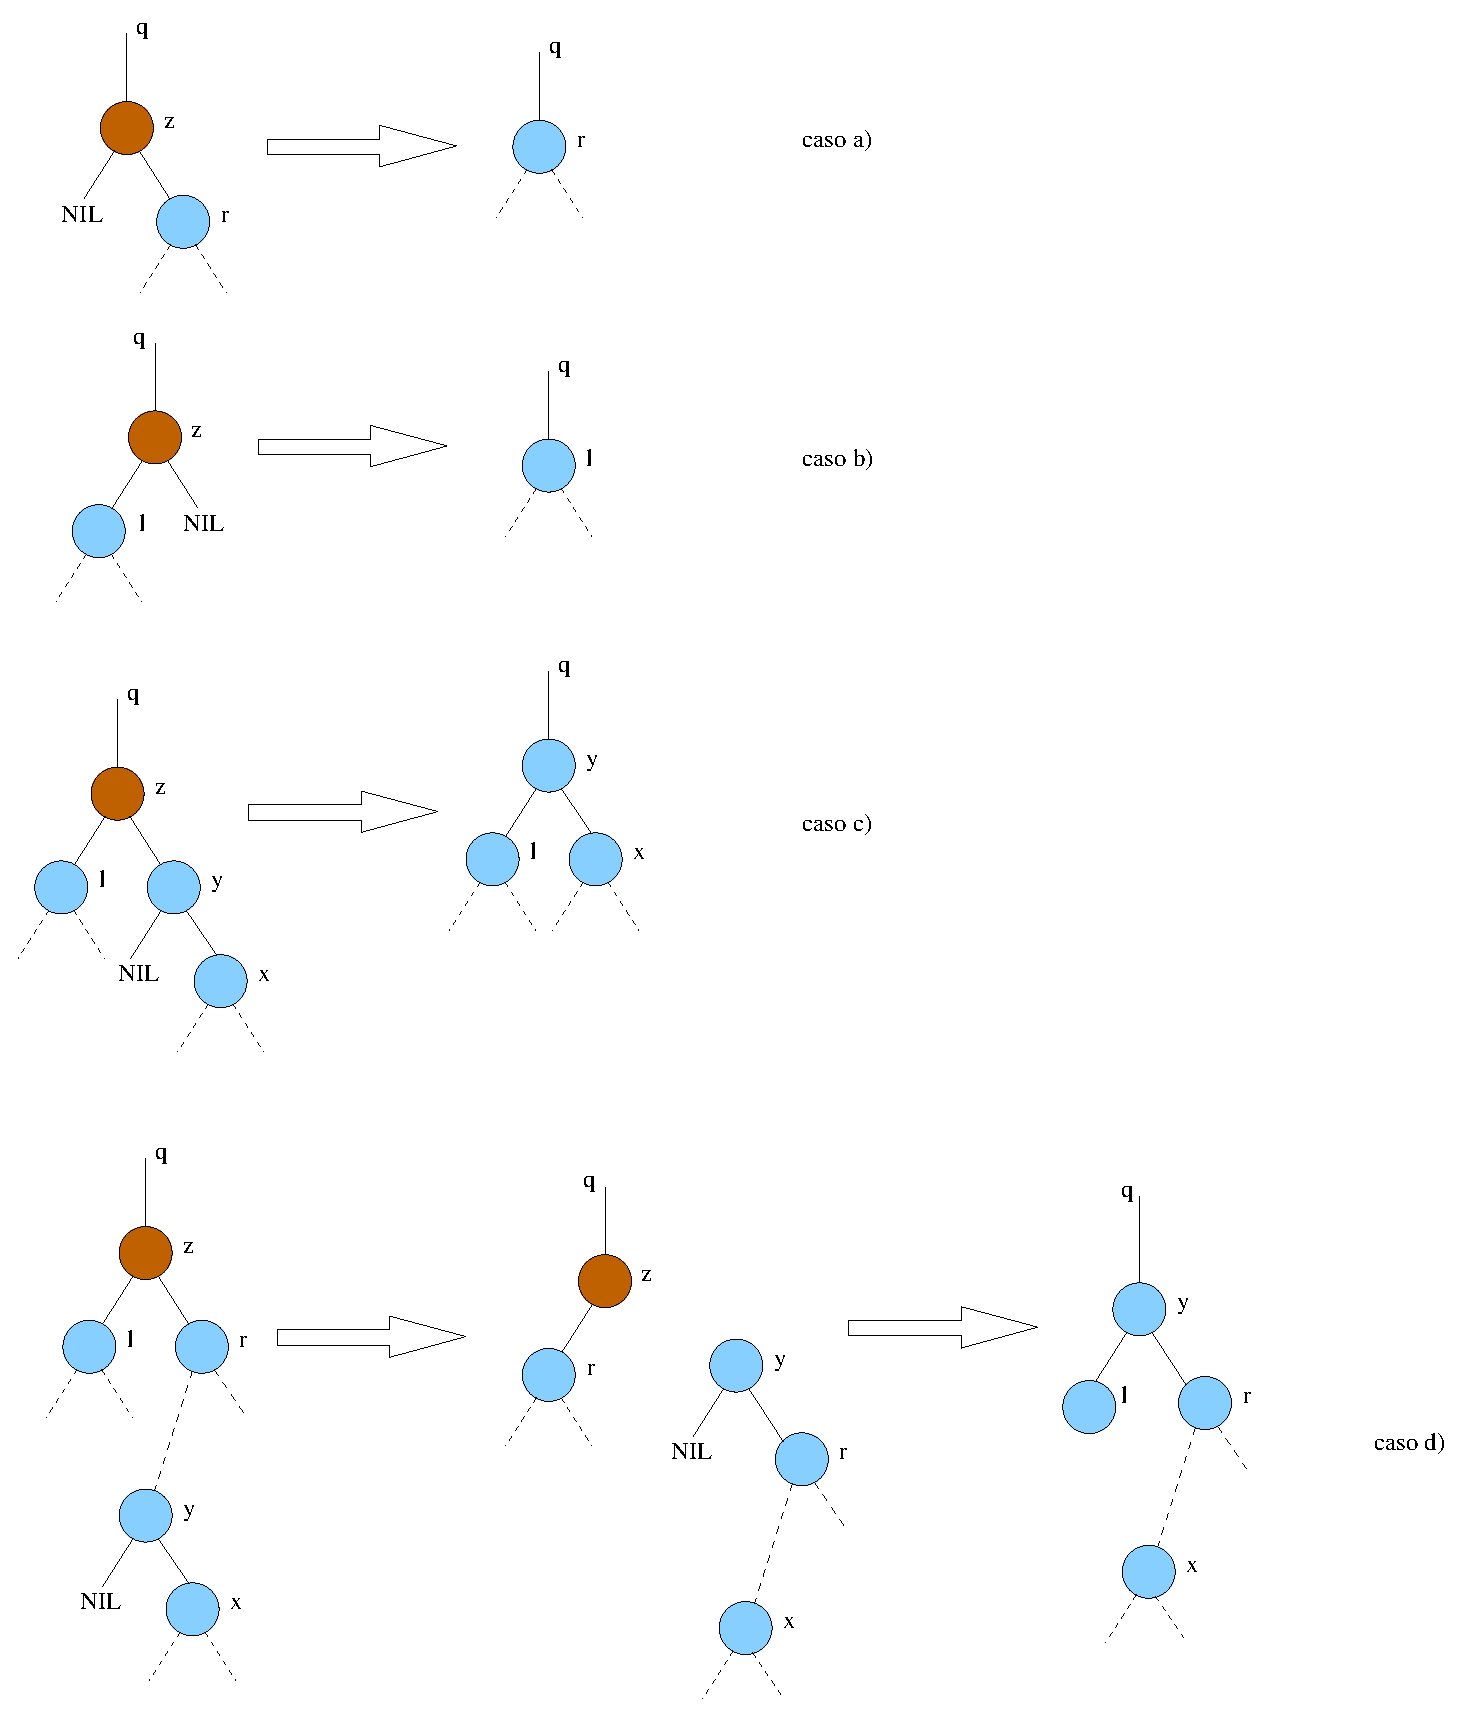
\includegraphics [width = 0.5\textwidth] {figs/node.tikz}

\end {document}


